%%%%%%%%%%%%%%%%%%%%%%%%%%%%%%%%%%%
%This is the LaTeX ARTICLE template for RSC journals
%Copyright The Royal Society of Chemistry 2016
%%%%%%%%%%%%%%%%%%%%%%%%%%%%%%%%%%%

\documentclass[twoside,twocolumn,9pt]{article}
\usepackage{extsizes}
\usepackage[super,sort&compress,comma]{natbib} 
\usepackage[version=3]{mhchem}
\usepackage[left=1.5cm, right=1.5cm, top=1.785cm, bottom=2.0cm]{geometry}
\usepackage{balance}
\usepackage{mathptmx}
\usepackage{sectsty}
\usepackage{graphicx} 
\usepackage{lastpage}
\usepackage[format=plain,justification=justified,singlelinecheck=false,font={stretch=1.125,small,sf},labelfont=bf,labelsep=space]{caption}
\usepackage{float}
\usepackage{fancyhdr}
\usepackage{fnpos}
\usepackage[english]{babel}
\addto{\captionsenglish}{%
  \renewcommand{\refname}{Notes and references}
}
\usepackage{array}
\usepackage{droidsans}
\usepackage{charter}
\usepackage[T1]{fontenc}
\usepackage[usenames,dvipsnames]{xcolor}
\usepackage{setspace}
\usepackage[compact]{titlesec}
\usepackage{hyperref}
%%%Please don't disable any packages in the preamble, as this may cause the template to display incorrectly.%%%


\usepackage{epstopdf}%This line makes .eps figures into .pdf - please comment out if not required.

\definecolor{cream}{RGB}{222,217,201}

% (RSC template bibliography preamble removed: it printed instructions into the reference list.)

\begin{document}

\pagestyle{fancy}
\thispagestyle{plain}
\fancypagestyle{plain}{
%%%HEADER%%%
\renewcommand{\headrulewidth}{0pt}
}
%%%END OF HEADER%%%

%%%PAGE SETUP - Please do not change any commands within this section%%%
\makeFNbottom
\makeatletter
\renewcommand\LARGE{\@setfontsize\LARGE{15pt}{17}}
\renewcommand\Large{\@setfontsize\Large{12pt}{14}}
\renewcommand\large{\@setfontsize\large{10pt}{12}}
\renewcommand\footnotesize{\@setfontsize\footnotesize{7pt}{10}}
\makeatother

\renewcommand{\thefootnote}{\fnsymbol{footnote}}
\renewcommand\footnoterule{\vspace*{1pt}% 
\color{cream}\hrule width 3.5in height 0.4pt \color{black}\vspace*{5pt}} 
\setcounter{secnumdepth}{5}

\makeatletter 
\renewcommand\@biblabel[1]{#1}            
\renewcommand\@makefntext[1]% 
{\noindent\makebox[0pt][r]{\@thefnmark\,}#1}
\makeatother 
\renewcommand{\figurename}{\small{Fig.}~}
\sectionfont{\sffamily\Large}
\subsectionfont{\normalsize}
\subsubsectionfont{\bf}
\setstretch{1.125} %In particular, please do not alter this line.
\setlength{\skip\footins}{0.8cm}
\setlength{\footnotesep}{0.25cm}
\setlength{\jot}{10pt}
\titlespacing*{\section}{0pt}{4pt}{4pt}
\titlespacing*{\subsection}{0pt}{15pt}{1pt}
%%%END OF PAGE SETUP%%%

%%%FOOTER%%%
\fancyfoot{}
\fancyfoot[LO,RE]{\vspace{-7.1pt}
\includegraphics[height=9pt]{head_foot/LF}}
\fancyfoot[CO]{\vspace{-7.1pt}\hspace{13.2cm}
\includegraphics{head_foot/RF}}
\fancyfoot[CE]{\vspace{-7.2pt}\hspace{-14.2cm}
\includegraphics{head_foot/RF}}
\fancyfoot[RO]{\footnotesize{\sffamily{1--\pageref{LastPage} ~\textbar  \hspace{2pt}\thepage}}}
\fancyfoot[LE]{\footnotesize{\sffamily{\thepage~\textbar\hspace{3.45cm} 1--\pageref{LastPage}}}}
\fancyhead{}
\renewcommand{\headrulewidth}{0pt} 
\renewcommand{\footrulewidth}{0pt}
\setlength{\arrayrulewidth}{1pt}
\setlength{\columnsep}{6.5mm}
\setlength\bibsep{1pt}
%%%END OF FOOTER%%%

%%%FIGURE SETUP - please do not change any commands within this section%%%
\makeatletter 
\newlength{\figrulesep} 
\setlength{\figrulesep}{0.5\textfloatsep} 

\newcommand{\topfigrule}{\vspace*{-1pt}% 
\noindent{\color{cream}\rule[-\figrulesep]{\columnwidth}{1.5pt}} }

\newcommand{\botfigrule}{\vspace*{-2pt}% 
\noindent{\color{cream}\rule[\figrulesep]{\columnwidth}{1.5pt}} }

\newcommand{\dblfigrule}{\vspace*{-1pt}% 
\noindent{\color{cream}\rule[-\figrulesep]{\textwidth}{1.5pt}} }

\makeatother

%%%TITLE, AUTHORS AND ABSTRACT%%%
\twocolumn[
  \begin{@twocolumnfalse}
{
\includegraphics[height=30pt]{head_foot/journal_name}\hfill\raisebox{0pt}[0pt][0pt]{
\includegraphics[height=55pt]{head_foot/RSC_LOGO_CMYK}}\\[1ex]

\includegraphics[width=18.5cm]{head_foot/header_bar}}\par
\vspace{1em}
\sffamily
\begin{tabular}{m{4.5cm} p{13.5cm} }


\includegraphics{head_foot/DOI} & \noindent\LARGE{\textbf{An open-source, 3D-printed auger powder doser designed with generative artificial intelligence$^\dag$}} \\
\vspace{0.3cm} & \vspace{0.3cm} \\

 & \noindent\large{Sam Charles,$^{\ast}$\textit{$^{a}$} Will Mulberry,\textit{$^{a}$} Luke Winters,\textit{$^{a}$} Carl Robinson,\textit{$^{a}$} Gage Erickson,\textit{$^{a}$} and Sterling G. Baird\textit{$^{b}$}} \\

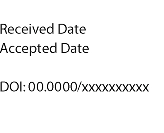
\includegraphics{head_foot/dates} & \noindent\normalsize{Weighing out powders is still largely done by hand, even in automated laboratories, because commercial powder-dosing robots cost tens to hundreds of thousands of dollars. We describe a single-channel powder doser built from 3D-printed parts and off-the-shelf electronics for under \$200, not counting the analytical balance it weighs into. A printed auger, a tube with a helical flight inside, carries powder to the outlet, and a \$6 microcontroller turns, tilts and taps it until the balance reads the requested mass. The mechanical parts were modelled by generative artificial intelligence (AI) rather than drawn in conventional CAD software: the team made every design decision and reviewed, printed and tested every part, while AI coding agents, and later a chat-driven CAD tool, produced the geometry. Asking the AI for the whole assembly at once failed repeatedly; asking for one part at a time, against dimensioned drawings, worked. We tested the doser on 13 powders, from table salt and food thickeners to an aluminium alloy powder and silicon. With one fixed set of settings, ten powders moved at 10--231~mg per auger revolution and three did not move at all. In closed loop, all 24 doses of 1~g on seven powders landed within $\pm$5\% of the target, and those of the three alloy-relevant powders within 1\%; doses of 50 and 200~mg were less reliable, because fast powders overshot and slow ones ran out of time. The design files, firmware, data and complete AI interaction history are public.} \\

\end{tabular}

 \end{@twocolumnfalse} \vspace{0.6cm}

  ]
%%%END OF TITLE, AUTHORS AND ABSTRACT%%%

%%%FONT SETUP - please do not change any commands within this section
\renewcommand*\rmdefault{bch}\normalfont\upshape
\rmfamily
\section*{}
\vspace{-1cm}


%%%FOOTNOTES%%%

\footnotetext{\textit{$^{a}$~Department of Mechanical Engineering, Brigham Young University, Provo, UT, USA. E-mail: TODO-corresponding-email}}
\footnotetext{\textit{$^{b}$~Department of Materials Science \& Engineering, University of Utah, Salt Lake City, UT, USA.}}

\footnotetext{\dag~Supplementary Information available: bill of materials, construction guide, auger and outlet cross-sections, bench noise record, closed-loop dose record, and AI usage log. See DOI: 00.0000/00000000.}

%%%END OF FOOTNOTES%%%

%%%MAIN TEXT%%%%

\section{Introduction}

Self-driving laboratories (SDLs) pair automated instruments with machine-learning planners that choose the next experiment, and they have sped up discovery in chemistry and materials science by an order of magnitude or more.\cite{Abolhasani2023Rise,Tom2024Self,Szymanski2023Autonomous,Seifrid2022Autonomous} Software for running them,\cite{Fei2024Alabos,Guzik2023Decade} methods for planning experiments,\cite{Baird2026Honegumi} and robots for handling liquids are now mature. Handling solids is not: most SDL demonstrations either work only with liquids or rely on a person to weigh out the powders.\cite{Maffettone2023What,Canty2025Science} The gap matters most where the powders are the experiment. In alloy discovery by additive manufacturing (AM, the 3D printing of metal parts), each candidate composition is made by blending elemental or pre-alloyed powders,\cite{Li2018Combinatorial,Vecchio2021Throughput,Moorehead2020Throughput,Mooraj2024Additive,Nelaturu2024Multi} so weighing many different powders accurately and repeatably is the step that limits the whole workflow.

Commercial powder-dosing systems exist and work well, but their cost and size put them out of reach of most academic laboratories. Benchtop gravimetric (weight-based) dispensers such as the METTLER TOLEDO XPR/CHRONECT line, Labman dosing stations and MTI's AM powder dispensers cost from tens of thousands to several hundred thousand dollars, are built around pharmaceutical and quality-control work, and usually dose one vial at a time from proprietary dosing heads.\cite{Besenhard2015Accuracy,Yang2007Metering} Pharmaceutical manufacturing meters powders at much higher flow rates with loss-in-weight feeders, which weigh the hopper continuously as it empties,\cite{Engisch2012Method,Engisch2015Feedrate,Hanson2018Control} and laboratory studies have dosed milligram quantities with capillaries, vibrating chutes and augers.\cite{Besenhard2017Micro,Faulhammer2014Dose,Chianrabutra2014Powder,Alsenz2011Powderpicking} None of these is available as an open design that a laboratory can print, build and modify. Open-source hardware has shown that 3D-printed instruments can reach research-grade performance at 1--10\% of the commercial price and keep improving through community contributions,\cite{Pearce2020Economic,Hohlbein2022Open,Wenzel2023Open,Stirling2022Hardops} and platforms such as Jubilee and low-cost SDL kits have brought that model to laboratory automation.\cite{Vasquez2020Jubilee,Subbaraman2024Duckbot}

This paper describes the first module of such an instrument: a single-channel powder doser in which a 3D-printed auger delivers powder into a cup on an analytical balance, and a microcontroller turns, tilts and taps the auger until the balance reads the requested mass (Fig.~\ref{fgr:overview}). Each channel is a self-contained printable unit, so later versions can arrange several channels around one cup to dose several powders (Section~\ref{sec:future}). We report the design, a test campaign on 13 powders with very different flow behaviour, and closed-loop dosing results, including where the current design fails.

The second contribution concerns how the doser was designed. No conventional CAD software, such as SolidWorks or Fusion~360, was used to design its parts. The mechanical parts were modelled by generative artificial intelligence instead: large language model (LLM) coding agents wrote each part as code in the project's public repository, and late in the project a chat-driven CAD tool, Zoo Design Studio, was used for the final parts. The division of labour was the same throughout. People decided what to build, wrote the specifications and, increasingly, supplied fully dimensioned drawings, and reviewed, printed and tested every part; the AI tools turned those decisions into geometry. Research on generative CAD has produced large datasets and models,\cite{Wu2021Deepcad,Willis2021Fusion,Seff2021Vitruvion,Xu2024Brepgen} and LLMs can now write CAD programs from written descriptions,\cite{Alrashedy2025Generating,Badagabettu2024Query2cad,Jansen2023Words,Rios2023Text} but published evaluations test benchmark shapes rather than the design of a working instrument from start to finish. Every prompt, generated part, review comment and failure in this project is preserved in a public repository,\footnote{All issue threads, pull requests and design-log entries cited in this paper are preserved at \url{https://github.com/vertical-cloud-lab/powder-doser}; ``the repository'' refers to this address throughout.} so the doser doubles as a documented case study of AI-assisted hardware design. We describe the workflow that eventually worked, the ways the AI tools failed, and what the approach cost and gained compared with conventional design.

\section{Results and discussion}

\subsection{The dosing module}

Fig.~\ref{fgr:overview}a,b shows the module as designed and as built. Powder is loaded through slots straight into the printed auger tube, which is also the reservoir; there is no separate hopper. The tube (25~mm outer diameter, 21~mm bore) is printed as one piece with an 8~mm central core and a single helical flight of 10~mm pitch, and the whole piece turns together, like an Archimedes screw, rather than as a screw inside a fixed barrel (Fig.~\ref{fgr:overview}c). A NEMA-11 stepper motor turns it through a printed 20-tooth pinion and a 44-tooth gear on the tube, a 2.2:1 reduction. Two further actuators help cohesive powders move: a push--pull solenoid that taps the tube through a printed collar, and a small eccentric-rotating-mass (ERM) vibration motor, the kind that makes a phone vibrate, mounted on the same collar. The tube rides on a hinged plate that two servos tilt through a 2:1 gear. Because the hinge axis passes through the outlet, the dose lands in the same place at every angle (Fig.~\ref{fgr:overview}d): the tube can be parked horizontally, where nothing flows, and tipped up to dispense. The hinge allows tilts up to vertical, but all tests in this paper used angles between horizontal and 45$^\circ$.

An analytical balance (A\&D HR-100A, 0.1~mg readability) weighs the collection cup and reports to a \$6 Raspberry Pi Pico~W microcontroller. The microcontroller runs a three-phase dosing procedure: fast continuous rotation, then small rotations, then single taps until the reading is within tolerance of the requested mass (Fig.~\ref{fgr:overview}e; Experimental). All structural parts are printed in PLA without supports, and the remaining parts are commodity items. The bill of materials comes to under \$200 for a single channel, excluding the balance, which most laboratories already own (SI Table~S1). That is roughly two orders of magnitude below a commercial gravimetric dosing head.

\begin{figure*}
 \centering
 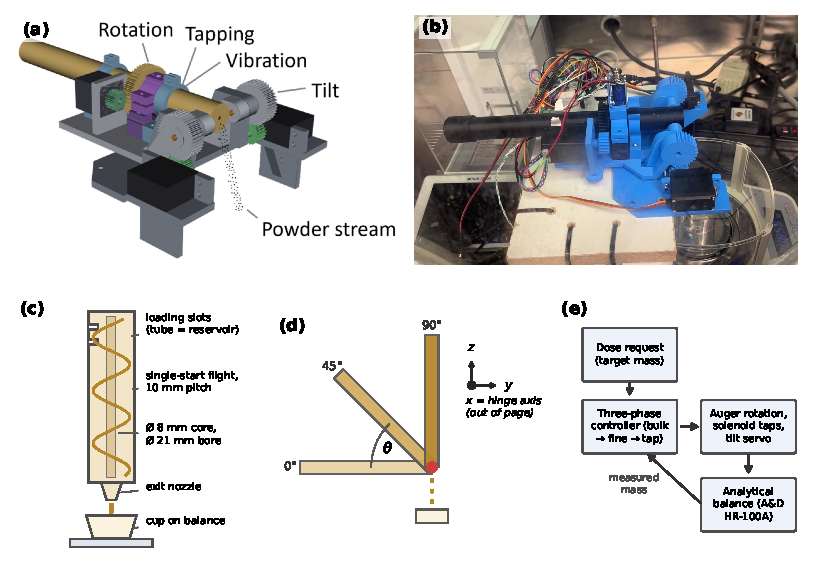
\includegraphics[width=17.1cm]{figures/fig1_overview}
 \caption{The single-channel powder doser. (a) Annotated CAD model, showing the four motions: auger rotation, tapping, vibration and tilt. (b) The module as built, photographed from the same viewpoint during its first automated dispense (sodium chloride into a crucible on the balance). (c) Powder path: powder is loaded through slots into the auger tube, which is itself the reservoir, and is carried down the helical flight to the outlet and into a cup on the balance. The tube, flight and core are printed as one piece and turn together. (d) Tilt about the fixed dispense point (red): the hinge axis $x$ passes through the outlet, so the dose lands in the same place as the tilt angle $\theta$ changes. The hinge allows 0$^\circ$ (horizontal park) to 90$^\circ$; the tests reported here used 0--45$^\circ$. (e) Closed-loop dosing: the controller compares the requested mass with the balance reading and drives the actuators until the two agree. Humans made every design decision and reviewed, printed and tested every part; AI tools produced the CAD models, and no conventional CAD software was used to design them.}
 \label{fgr:overview}
\end{figure*}

\subsection{How the parts were designed}

The mechanical design went through four generations in six weeks, recorded step by step in a 97-entry design log in the repository. The project began as a hand-sketched mechanical scoop (a ``powder excavator'') meant to ride on an existing computer-controlled (CNC) gantry. An AI-assisted survey of small-scale dosing mechanisms\cite{Besenhard2017Micro,Faulhammer2014Dose} produced a list of eight candidates, among them a tap sieve, a metering wheel, a capillary wiper and an auger. The team chose the auger for its dose resolution, its printability and its tolerance of different powders, in line with its wide use in commercial micro-feeders.\cite{Yang2007Metering,Besenhard2015Accuracy} The second generation packaged the auger, frame, drive and actuators as a self-contained channel, the repeating unit of a future multi-powder doser. The third generation changed the method rather than the mechanism. Instead of asking the AI tools for the whole module at once, the team specified each part separately (auger, geared auger, bracket, tap collar, mounting plate, baseplate and servo hinge), and each was modelled, reviewed and printed on its own. The fourth generation assembled these parts on the hinged baseplate with servo tilt. Four printed outlet geometries were also made (SI Fig.~S1).

The specifications given to the AI grew steadily more detailed. Early requests described what a part had to do and how it met its neighbours: bolt patterns, shaft diameters and mating faces. Later the team supplied annotated engineering drawings, several of them fully dimensioned with the geometric relations between features. By the end, the AI's job had narrowed to modelling, that is, turning drawings into parametric CAD and working out derived dimensions and clearances. Every design decision stayed with the team.

Most parts were produced by LLM coding agents (the GitHub Copilot coding agent, mainly running Claude-family models) working directly in the repository. Given a task written as a GitHub issue, the agent wrote the part as parametric code (Python with build123d or CadQuery, or OpenSCAD). Automated checks that run on every change (continuous integration) then rendered views of the part and exported printable STL mesh files, and the agent opened a pull request that the team reviewed from the rendered images. Two commercial text-to-CAD services were tried on the same parts: CADSmith, and Zoo Design Studio, which pairs a code-based CAD engine, scripted in the KittyCAD Language (KCL), with a conversational design agent called Zookeeper. Zoo Design Studio was adopted for the final parts, and even there parts were built mainly by chatting with the agent rather than by editing the model by hand. Every prompt, generated file, render and review comment is preserved in the repository's pull requests and in a dedicated discussion thread.

\begin{figure*}
 \centering
 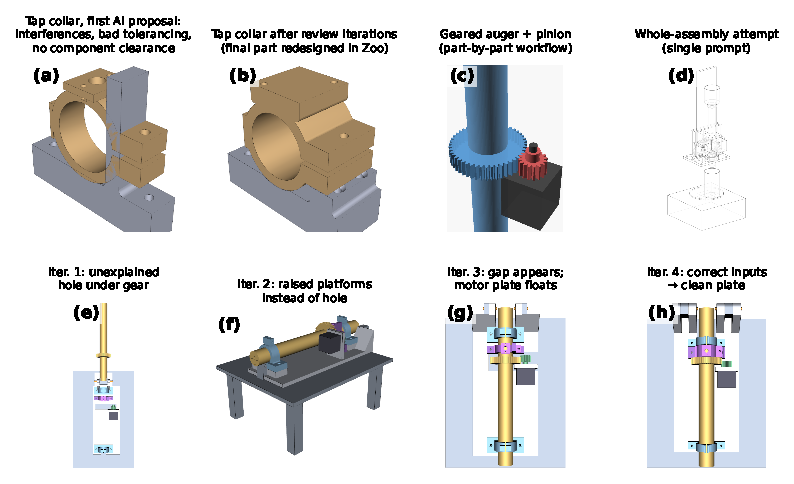
\includegraphics[width=17.1cm]{figures/fig2_genai}
 \caption{AI-generated CAD, good and bad. (a) The first AI-generated tap collar: several functions merged into one body, with features overlapping one another, wrong tolerances, no room for the solenoid and vibration motor it had to carry, and no workable spatial layout. It could not have been built. (b) The same part after iterative review with the coding agent; the production collar was later remodelled in Zoo Design Studio, which reached a usable part in three iterations. (c) Geared auger and stepper pinion from the part-by-part workflow. (d) An attempt to generate the whole module from a single prompt: plausible at a glance, but with overlapping solids and floating parts that took longer to diagnose than the part-by-part route took to build. (e--h) Four review iterations of the mounting plate. The agent added an unexplained hole (e), then raised platforms (f), then a gap that left the motor plate floating (g), and produced a clean plate (h) only once the correct versions of the neighbouring parts were supplied. The cause was out-of-date input files, a human error that the agent silently designed around. All parts shown were modelled by AI tools to human-set requirements and reviewed by the team at each iteration; no conventional CAD software was used.}
 \label{fgr:genai}
\end{figure*}

\paragraph{One part at a time.~~} Early attempts asked the agent for the complete module from a description of its layout. The results looked plausible and did not work. The first tap collar merged several functions into one body, with overlapping features, wrong tolerances and no room for the actuators it existed to carry (Fig.~\ref{fgr:genai}a). An early bracket arrived with its two mounting plates unconnected. Requests at the level of the assembly repeatedly produced overlapping solids, floating parts and changes nobody had asked for, and fixing one defect often introduced another (Fig.~\ref{fgr:genai}d). Restricting each request to a single part, with its interfaces listed explicitly, turned the agent into a productive collaborator (Fig.~\ref{fgr:genai}c). This fits the known weakness of current LLMs at reasoning about how shapes fit together in space,\cite{Alrashedy2025Generating} and it suggests that splitting a design into parts with defined interfaces, standard practice for human engineers, is currently required rather than optional when AI does the modelling. Table~\ref{tbl:aifail} lists the failure modes we met and what caught each one. Each design-log entry records what triggered the change, the reasoning and the outcome (built and worked, built with issues, failed, or superseded); a quantitative analysis of the log is planned for the multi-doser follow-up.

\begin{table}[h]
\small
  \caption{\ Failure modes of the AI modelling tools observed in this project, and what caught or prevented each one.}
  \label{tbl:aifail}
  \begin{tabular*}{0.48\textwidth}{@{\extracolsep{\fill}}p{2.3cm}p{2.9cm}p{2.6cm}}
    \hline
    Failure & Example & Caught or prevented by \\
    \hline
    Parts that do not fit together & Whole-module prompts; first tap collar; bracket with unconnected plates (Fig.~\ref{fgr:genai}a,d) & Asking for one part at a time, with interfaces listed \\
    Unrequested changes & Fixing one defect altered an unrelated feature & Full re-inspection of rendered views at every iteration \\
    Mislabelled variants & Two of four test nozzles swapped relative to their documentation & Human cross-check before printing \\
    Sub-millimetre errors & Height mismatch of one print layer & Only the failed print \\
    Designing around bad inputs & Out-of-date neighbouring parts led to a hole, platforms, then a gap (Fig.~\ref{fgr:genai}e--h) & Supplying the correct upstream files \\
    No sense of ``finished'' & Late iterations disturbed features that were already right & The team freezing the geometry \\
    Wrong orientation & Solenoid mis-oriented on the tap collar over several coding-agent iterations & Switching the part to Zoo Design Studio \\
    \hline
  \end{tabular*}
\end{table}

\paragraph{Checking the output.~~} Most of the effort went into checking. Because any iteration could change geometry outside the part being edited, every generated part had to be re-inspected in full. In one case the agent produced four miniature test nozzles and swapped the labels on two of them, which would have invalidated a dispensing comparison had a person not noticed. Automated checks (that a part is a single solid, that its surface has no holes, and that key interface dimensions are correct) caught a useful share of defects cheaply. Small errors still escaped both the checks and visual review: a height mismatch of one print layer was found only when the part peeled off the print bed. One pattern held across the project. AI-generated alternatives were valuable early, while the design was still open, but late in the project the agent could not tell how close a part was to finished and kept changing features that were already right. AI-modelled parts therefore tended to stop at ``good enough'', because each further round of edits cost time and risked breaking something that worked.

\paragraph{Comparing the tools.~~} The coding-agent workflow was fully traceable and needed nothing beyond a web browser, but each iteration took minutes and every change had to be reviewed. CADSmith converged quickly on brackets and plates once given the same interface specifications. Zoo Design Studio, tried last, was the team's clear favourite. Its Zookeeper agent reasoned noticeably better about space, ran its own checks (such as counting solid bodies) before returning a result, and worked inside a live CAD view, so the team could inspect an editable model as it was built. Each iteration was slower, of the order of an hour, but one or two Zoo iterations achieved what took seven or eight with the coding agent. The final tap collar reached a usable design in three Zoo iterations after the same number of coding-agent iterations had failed to orient the solenoid correctly. At the time of testing, Zoo's limits mirrored its strengths: imported reference parts could not be edited, there were no constraints between parts in an assembly, and manual edits were largely limited to changing parameter values, so the work stayed conversational. These rankings are the team's impressions from one project, not measurements; a controlled comparison with identical prompts and parts is planned. The team also agreed that every AI route was slower, and gave lower-quality geometry, than experienced mechanical engineers working in conventional CAD software would have. As a rough check, a team member later re-modelled nine of the AI-designed parts by hand in Fusion~360; the edited recordings total about three hours, about as long as a single Zoo Design Studio session. What the AI route bought instead was documentation as a by-product of the work. Every design intent, constraint and revision exists as text, which makes the design reproducible, its history traceable and the project easy to hand over, in a way that conventional CAD files are not.

\subsection{How much powder one turn delivers}

We tested the doser on 13 powders (Table~\ref{tbl:powders}). Seven are food-safe surrogates, chosen to cover a wide range of flow behaviour cheaply and safely: table salt (NaCl, the control), calcium lactate, xanthan gum, carboxymethyl cellulose (CMC), sodium alginate, and white and brown rice flour. The other six are relevant to the alloy-discovery work the doser is meant to serve: a gas-atomized AlSi10Mg alloy powder (near-spherical particles made by spraying molten metal), a coarse and a fine grade of silicon, sodium sulfate, barium chloride, and fumed silica, a very light flow aid. Each powder went through the same fixed sequence of test protocols with frozen settings (Table~\ref{tbl:protocols}), so that differences between powders reflect the powders rather than the settings. In the first test round (4--21 August 2026), the food-safe powders were tested on an open laboratory bench and the other powders in a shared fume hood. The balance became much noisier from 20 August: with nothing moving, eight successive readings varied by 0.0~mg on every run up to 12 August and by up to 88~mg afterwards (SI Fig.~S2). Bench conditions are therefore confounded with powder group, because every research-relevant powder was measured in the noisier period. The noise was later traced to powder trapped under a misaligned dust plate on the balance; after cleaning, the balance drifted by less than 0.1~mg over 16 minutes. All data in this paper were recorded before that fix.

\begin{table*}[t]
\small
  \caption{\ The 13 powders tested. Mass per auger revolution is the protocol~C mean at 22.5$^\circ$ tilt (Fig.~\ref{fgr:conveyance}a). Closed-loop columns give the number of valid doses that finished within the acceptance limit ($\pm$10\% at 50~mg, $\pm$5\% at 200~mg and 1~g) out of the number run (Fig.~\ref{fgr:closedloop}); a dash means not run. The silicon grades are named by sieve size: $-$325 mesh passes a 44~$\mu$m sieve, and $-$110/+200 mesh lies between about 75 and 150~$\mu$m.}
  \label{tbl:powders}
  \begin{tabular*}{\textwidth}{@{\extracolsep{\fill}}llrccc p{5.2cm}}
    \hline
    Powder & Group & mg per rev. & 50~mg & 200~mg & 1~g & Observed behaviour \\
    \hline
    AlSi10Mg (gas-atomized) & Research & 231 & 1/3 & 3/3 & 3/3 & Fastest powder; fluid-like; overshoots small targets \\
    Silicon, $-$110/+200 mesh & Research & 211 & 2/2 & 2/3 & 3/3 & Free-flowing \\
    Sodium sulfate & Research & 208 & 0/3 & 2/3 & 3/3 & Free-flowing; overshoots small targets \\
    Calcium lactate & Surrogate & 198 & 1/2 & 2/3 & 3/3 & Free-flowing; largest tap increment \\
    Barium chloride & Research & 185 & -- & -- & -- & Absorbed moisture and caked in the tube in round 2 \\
    Xanthan gum & Surrogate & 161 & 2/3 & 3/3 & 3/3 & Flows under rotation; can clog after bursts \\
    Sodium chloride (control) & Surrogate & 146 & 2/3 & 2/3 & 6/6 & Free-flowing baseline \\
    Carboxymethyl cellulose & Surrogate & 26 & 3/3 & 1/3 & 3/3 & Slow; charges electrostatically \\
    White rice flour & Surrogate & 13 & 3/3 & 3/3 & 0/3 & Slow and pulsing; most variable between revolutions \\
    Sodium alginate & Surrogate & 10 & 0/3 & 0/3 & 0/3 & Slowest powder that moved \\
    Silicon, $-$325 mesh & Research & none & 0/3 & 0/3 & 0/6 & Did not move at 0 or 22.5$^\circ$; one pulse at 45$^\circ$ \\
    Brown rice flour & Surrogate & none & -- & -- & 0/3 & Did not move at any tilt \\
    Fumed silica & Research & none & -- & -- & -- & Did not move; very light and fluffy \\
    \hline
  \end{tabular*}
\end{table*}


\begin{table*}[t]
\small
  \caption{\ Test protocols. Every powder went through the same protocols in the same order with frozen settings, so results can be compared across powders; the sequence characterizes the powders and does not tune anything. Rotations and speeds refer to the auger; tilts are the tube's angle above horizontal (the firmware records them as 0, 45 and 90, see Experimental). A trial is one recorded measurement.}
  \label{tbl:protocols}
  \begin{tabular*}{\textwidth}{@{\extracolsep{\fill}}p{2.6cm}p{2.5cm}p{5.0cm}p{5.2cm}l}
    \hline
    Protocol & Varied & Fixed settings & What it measures & Trials \\
    \hline
    A \ Balance baseline & Nothing & Tilt 22.5$^\circ$; eight readings, no actuation & Noise floor of the run, against which every other protocol is read & 8 \\
    B \ Static hold & Tilt (0, 22.5, 45$^\circ$) & 15~s hold at each tilt, no actuation & Whether any powder flows on its own (clean shut-off) & 3 \\
    C \ Rotation & Tilt (0, 22.5, 45$^\circ$) & Six single revolutions per tilt at 30~rpm, with a settled reading after each & Mass per revolution and its revolution-to-revolution variation & 18 \\
    D \ Speed sweep & Speed (15, 45, 90~rpm) & Tilt 22.5$^\circ$; three revolutions commanded per speed; balance streamed every 0.25~s & Delivery rate against speed; mass-against-time traces & 3 \\
    E \ Tap & Tilt (0, 22.5$^\circ$) & Eight trials of a one-revolution re-feed followed by one 60~ms solenoid tap & Mass released by a single tap, with the re-feed logged separately & 32 \\
    F \ Vibration & Tilt (0, 22.5$^\circ$) & As E, with three vibration bursts in place of the tap & Mass released by vibration (no data: driver fault) & 0 \\
    G \ Closed-loop, 1~g & Nothing & Three doses of 1.000~g; three-phase controller & Dose error, time and effort per phase & 3 doses \\
    H \ Closed-loop, small & Target (50, 200~mg) & Three doses at each target; same controller & Dose error and time at small targets & 6 doses \\
    \hline
  \end{tabular*}
\end{table*}


With one set of settings, the mass delivered per auger revolution at a 22.5$^\circ$ tilt varied 24-fold across the ten powders that moved, from 10~mg for sodium alginate to 231~mg for AlSi10Mg (Fig.~\ref{fgr:conveyance}a). Seven powders (AlSi10Mg, coarse silicon, sodium sulfate, calcium lactate, barium chloride, xanthan gum and salt) delivered 146--231~mg per revolution, and CMC, white rice flour and sodium alginate delivered 10--26~mg. Three powders did not move at any tilt: brown rice flour, fine silicon and fumed silica. The powder mattered far more than the settings. Of the variation in mass per revolution across all measured revolutions (on a log scale), 70\% was explained by which powder was loaded, 20\% by tilt, 4\% by the combination of the two, and 6\% was scatter from one revolution to the next.

\begin{figure*}
 \centering
 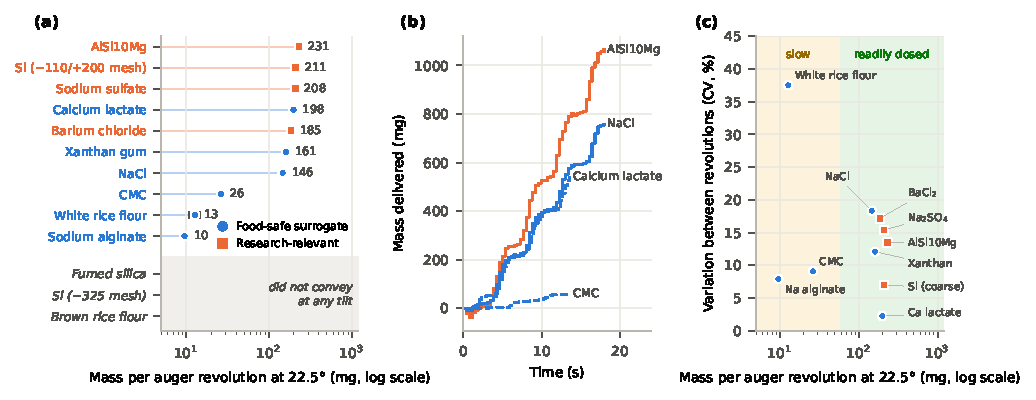
\includegraphics[width=17.1cm]{figures/fig3_conveyance}
 \caption{How much powder the auger delivers, for 13 powders under one fixed set of settings. (a) Mass delivered per auger revolution at 22.5$^\circ$ tilt (protocol C: six revolutions at 30~rpm; error bars show the standard error). The three powders at the bottom delivered nothing distinguishable from zero at any tilt and are listed without a value. (b) Balance readings streamed while the auger turned continuously at 15~rpm and 22.5$^\circ$ tilt (protocol D), for four powders. The mass rises in steps about 4~s apart, one per auger revolution. (c) Mass per revolution against the variation between successive revolutions (coefficient of variation of six revolutions). Both numbers come from protocol C alone; the shading marks the two groups discussed in the text. Blue circles are food-safe surrogates and orange squares research-relevant powders; one run per powder is shown (Experimental). Fill level was not controlled, particle size and shape were not measured, and all research-relevant powders were tested in the noisier period. Rotations and speeds refer to the auger, and angles to the tube's tilt above horizontal.}
 \label{fgr:conveyance}
\end{figure*}

Delivery is not smooth. Balance readings streamed during continuous rotation rise in steps (Fig.~\ref{fgr:conveyance}b) that recur about every 4~s at 15~rpm, once per auger revolution; across ten powders, the median period from autocorrelation was 3.94~s against a revolution time of 4.00~s. This is what a single-start flight should do: each revolution carries one pocket of powder over the outlet. The pulsing limits how finely rotation alone can meter powder, and it is why the final approach to a requested mass uses taps (Section~\ref{sec:closedloop}).

Plotting each powder's throughput against its variation from one revolution to the next (Fig.~\ref{fgr:conveyance}c) separates the powders into a readily dosed group, which delivers 150--230~mg per revolution with 2--18\% variation, and a slow group that delivers 10--26~mg. Both numbers come from about two minutes of bench time per powder, which makes the plot a candidate for sorting new powders quickly. For now it is a grouping rather than a validated diagnostic, because we have not independently measured particle size, particle shape or bulk density.

The two ends of the range are consistent with particle shape. Gas-atomized AlSi10Mg consists of near-spherical particles in a narrow size range, the properties laser powder-bed fusion requires, and it was the fastest powder tested. The fine silicon is milled, angular and smaller than 44~$\mu$m (it passes a 325-mesh sieve). It did not move at all at 0$^\circ$ or 22.5$^\circ$, and at 45$^\circ$ it produced a single 7~mg pulse in six revolutions. The coarse silicon, the same material at roughly 75--150~$\mu$m, delivered 211~mg per revolution. Forces that make particles stick together matter more relative to their weight as particles get smaller, which fits this sharp difference between the two silicon grades. We read the three powders that did not move as a limit of this auger geometry rather than a fixed property of the powders; a wider flight, a larger pitch or a taller fin would move that limit. The failures also differ in kind. Fine silicon moved slightly at the steepest tilt, so for it the driving force was too weak to overcome cohesion. Fumed silica, which is extremely light and fluffy, never delivered more than a few milligrams per revolution at any tilt and varied wildly between turns, which points instead to trapped air.

\subsection{Tilt and tapping}

Tilt was the strongest setting the controller has. For the nine powders measured at all three angles, raising the tube from horizontal to 22.5$^\circ$ increased delivery by a median factor of 4.2, and raising it further to 45$^\circ$ added a median factor of 1.2 (Fig.~\ref{fgr:knobs}a). The cohesive powders depended most on gravity: sodium alginate delivered 15 times more per revolution at 45$^\circ$ than horizontally and white rice flour 10 times more, against about 5 times for calcium lactate and sodium sulfate. Tilt was also the only setting that moved one of the non-conveying powders at all (fine silicon, at 45$^\circ$).

With the auger stopped, nothing flowed on its own. In 33 fifteen-second holds, covering all three tilts on the 11 runs recorded up to 12 August, the balance reading changed by 0.0~mg every time (protocol B). From 20 August, hold readings scattered by tens of milligrams in both directions, including at 0$^\circ$ where gravity cannot empty the tube, so they reflect the bench rather than the powder. Parking the tube horizontally therefore gives a clean shut-off.

\begin{figure*}
 \centering
 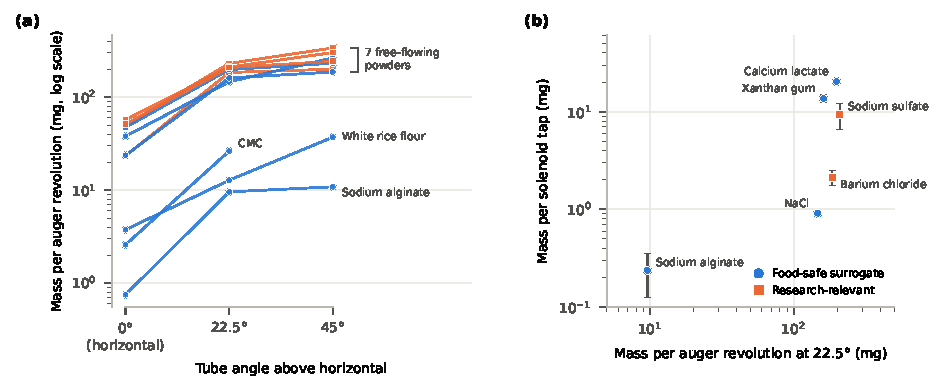
\includegraphics[width=17.1cm]{figures/fig4_knobs}
 \caption{Effect of tilt and tapping. (a) Mass per auger revolution with the tube horizontal and tilted to 22.5$^\circ$ and 45$^\circ$ (protocol C) for the ten powders that moved. Points are shown only where the mean exceeds twice its standard error, which CMC at 45$^\circ$ did not. The seven free-flowing powders overlap at the top and are bracketed; Table~\ref{tbl:powders} gives their values. On the logarithmic axis, equal vertical distances are equal ratios. (b) Mass released by one solenoid tap (protocol E; mean and standard error of eight taps at 22.5$^\circ$) against mass per auger revolution, for the six powders whose tap increment exceeded twice its standard error. Markers as in Fig.~\ref{fgr:conveyance}.}
 \label{fgr:knobs}
\end{figure*}

A single solenoid tap released between 0.2~mg (sodium alginate) and 20~mg (calcium lactate), or 0.6--10\% of one revolution's delivery (Fig.~\ref{fgr:knobs}b). The size of a tap does not simply follow throughput. Barium chloride and calcium lactate delivered similar amounts per revolution (185 and 198~mg) but released 2.1 and 20~mg per tap, a tenfold difference. Tap increments could be resolved only on the quieter runs; on most fume-hood runs they were smaller than the bench noise.

The vibration motor could not be characterised. Its driver (DRV2605L) returned an input/output error in every run that asked for protocol F, so no vibration data exist, and the doser as tested relies on rotation, tilt and tapping alone. The speed sweep (protocol D) suggests that delivery rate grows more slowly than speed. Fitting rate $\propto$ speed$^{\alpha}$ over 15--90~rpm gave a median $\alpha$ of 0.78 across ten powders, with three cohesive powders above 1 (white rice flour 1.36, CMC 1.13 and sodium alginate 1.08). We do not plot these results. Each speed was measured once, always in the same order, without re-zeroing the balance in between, and a firmware timing error let the auger turn 15--54\% further than commanded. The sweep will be repeated once these problems are fixed.

\subsection{Closed-loop dosing}
\label{sec:closedloop}

The controller doses in three phases: continuous rotation until the cup is within 0.5~g of the requested mass, then 45$^\circ$ rotations with a settled balance reading after each, and finally pairs of solenoid taps until the reading is within $\pm$5~mg (Experimental). All doses used one set of phase settings, tuned by hand on salt and frozen for every powder. In the first test round we ran three doses of 1~g (protocol G) on each powder whose bench conditions allowed it. A second round, from 3 to 15 September 2026, added three doses each of 50~mg and 200~mg (protocol H) and the 1~g doses that bench noise had prevented for the research-relevant powders. Doses are scored against acceptance limits fixed before testing: $\pm$10\% of the requested mass below 100~mg and $\pm$5\% at or above it. These limits were chosen so that dosing error adds less than one atomic percent of composition error to a typical five-component alloy blend.\cite{Vecchio2021Throughput,Moorehead2020Throughput} Failed doses stay in every count.

At 1~g, every dose of the seven free-flowing and moderately slow powders finished within the $\pm$5\% limit, 24 of 24 across salt, calcium lactate, xanthan gum, CMC, AlSi10Mg, coarse silicon and sodium sulfate (Fig.~\ref{fgr:closedloop}c). The three research-relevant powders were the most accurate: all nine of their 1~g doses finished within 10~mg (1\%) of the target, with a median time of 111~s. The four powders that failed at 1~g failed for two different reasons. Fine silicon and brown rice flour delivered nothing, as they had in the open-loop tests. White rice flour and sodium alginate did move, but too slowly: they used up the controller's budget of 200 small rotations and stopped 14\% and 29\% short of the target after about 14 minutes.

Smaller doses were harder, in different ways for fast and slow powders (Fig.~\ref{fgr:closedloop}a,b). At 200~mg, 18 of 30 doses finished within $\pm$5\%, including all three for AlSi10Mg, xanthan gum and white rice flour. At 50~mg, 14 of 28 finished within $\pm$10\%. The fast powders now overshot: of the 12 doses on free-flowing powders that missed the limit at 50 or 200~mg, 11 were overshoots, including all three sodium sulfate doses at 50~mg. For these powders the smallest rotation the controller takes already delivers a large fraction of a 50~mg dose, and delivery arrives in pulses (Fig.~\ref{fgr:conveyance}b), so the last increment can overshoot before the balance reading catches up. Slow powders undershot instead, for the same reason as at 1~g. Overshoot cannot be undone in powder dosing, so for small targets a finer final increment matters more than a faster one.

Time was the main cost of accuracy (Fig.~\ref{fgr:closedloop}d). Doses that finished within the limit took a median of 53~s at 50~mg, 152~s at 200~mg and 185~s at 1~g, far longer than the 30~s we had aimed for. Slow powders took much longer: white rice flour needed 11--13 minutes for each 200~mg dose. The fastest ``doses'' were failures: fine silicon and brown rice flour stopped after 6--52~s, when the controller detected that nothing was arriving.

Two features of the controller explain most of the remaining failures. First, it never returns to an earlier phase. Once the tap phase begins, it cannot rotate the auger to refill the outlet, apart from 5$^\circ$ nudges that proved too small for the slower powders; when the flight nearest the outlet runs empty, taps alone cannot finish the dose. This is how the first-round 1~g doses of calcium lactate, xanthan gum and CMC ended: each came to rest 15--49~mg short after 66--166 taps, inside the acceptance limit but outside the controller's own stopping band. Second, that stopping band was $\pm$5~mg at every target. At 1~g it is ten times tighter than the $\pm$50~mg acceptance limit, so the firmware logged these doses as stalled although they met the specification. We report every dose against the acceptance limit and keep the firmware's own label in the dose record (SI Table~S2). A controller that can return to rotation when taps stop working, and whose stopping band scales with the target, is the most direct improvement.

\begin{figure*}
 \centering
 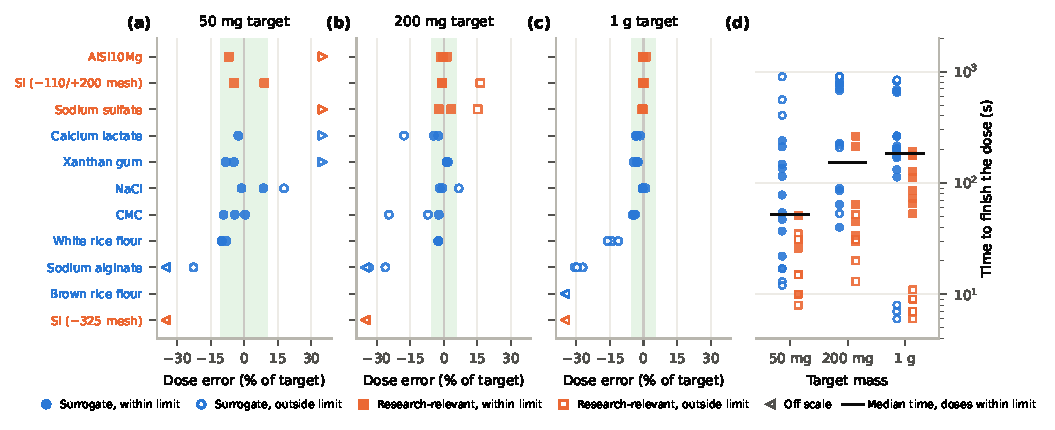
\includegraphics[width=17.1cm]{figures/fig5_closed_loop}
 \caption{Closed-loop dosing with one frozen set of controller settings. (a--c) Error of each valid dose at 50~mg, 200~mg and 1~g targets, as a percentage of the target. Green bands mark the acceptance limits ($\pm$10\% below 100~mg, $\pm$5\% at or above). Filled markers finished within the limit and open markers outside it; triangles at the edge are off scale (the powders that delivered little or nothing). Replicates share a row and are not jittered. Powders are ordered by mass per revolution (Fig.~\ref{fgr:conveyance}a). Doses at 1~g for the food-safe powders are from the first test round (protocol G, August 2026); all 50 and 200~mg doses and the 1~g doses for AlSi10Mg, coarse silicon and sodium sulfate are from the second round (protocols G and H, September 2026). Barium chloride has no valid closed-loop dose (it caked in the tube) and fumed silica was not dosed. (d) Time to finish each dose; horizontal bars are medians of the doses within the limit.}
 \label{fgr:closedloop}
\end{figure*}

\subsection{Limits of the current design}

Several limits follow from these results. First, the design covers doses from tens of milligrams to grams. Doses of 0.1--10~mg, which some chemistry applications need, are out of reach for now; they would require per-powder calibration, better isolation from vibration and a smaller auger. Second, three of the 13 powders did not move, so the current geometry sets a floor on how cohesive or how light a powder can be. Third, the outcome of a dose depends on where the powder happens to sit in the flight when the dose starts. There is no defined starting state, and in routine use the auger would never be reset between doses anyway, so this variability is part of the real performance. Fourth, all masses are what landed in the cup, not what left the tube; powder that missed the cup is not counted, and the tube's fill level was not controlled. Finally, the bench sets the noise floor. Most of the noise in this campaign came from powder trapped under the balance's dust plate, which has since been fixed, so the closed-loop results here are likely to understate what the doser can do on a clean balance.

\subsection{Cost and accessibility}

The single-channel module (printed parts, motors, drivers and microcontroller) costs under \$200 in single quantities, excluding the balance (SI Table~S1), and prints in under 24~h on a consumer printer. Commercial automated gravimetric dosing modules are quoted at \$30k--\$300k depending on configuration. Even where commercial instruments are more accurate, a cost gap of two orders of magnitude changes what a laboratory can do. It can dedicate one printed channel to each powder so that powders never mix, throw away and reprint the parts the powder touches, and replace a failed channel within a day. This is the economic argument for open-source laboratory hardware\cite{Pearce2020Economic,Hohlbein2022Open} applied to the solid-handling gap in SDLs.

\section{Experimental}
\label{sec:methods}

\subsection{Fabrication}
All printed parts were made in PLA on a Bambu Lab H2D printer (0.2~mm layers, four perimeters, 25\% infill). The auger is a single printed piece: a tube with 25~mm outer diameter and 21~mm bore, an 8~mm central core, a single-start helical flight 2~mm thick with 10~mm pitch, four 4~$\times$~7~mm loading slots in the tube wall, a tapered outlet with a 3~mm exit hole, and a gear band on the outside of the tube. As built, a 20-tooth pinion on the stepper drives a 44-tooth gear on the auger (2.2:1 reduction), and the servos drive the tilt plate through a 2:1 gear. The auger, gears, bracket, tap collar, mounting plate, hinged baseplate and servo gear sector are parametric models; their source files (build123d, OpenSCAD and KCL), printable STL files and renders for every iteration are in the repository. Purchased parts: a NEMA-11 stepper motor (auger drive), two MG996R-class servos (tilt), a 12~V push--pull solenoid (tapping), a coin-type ERM motor (vibration) and an A\&D HR-100A analytical balance (0.1~mg readability). The auger turns in printed collars rather than bearings.

\subsection{Electronics and firmware}
A Raspberry Pi Pico~W runs MicroPython firmware with commands to rotate by a given angle, tap, vibrate, tilt to an angle and read the mass. A Pololu Tic T500 drives the stepper over a serial (UART) link, a DRV8871 H-bridge drives the solenoid, and a DRV2605L haptic driver runs the vibration motor over I$^2$C; the balance is read over RS-232 through an SP3232 transceiver board. The electronics began on a breadboard and now sit on a custom printed circuit board (PCB). Schematics, board files, the wiring guide and the firmware are in the repository (\texttt{hardware/}).

The dosing firmware includes both gear ratios, so its rotation commands and records are in auger revolutions, auger rpm and plate degrees. The one exception is the test battery's tilt setting, which follows an older convention in which 90 meant the ``vertical'' preset: the battery records tilts of 0, 45 and 90, which the 2:1 servo gear turns into tube angles of 0$^\circ$, 22.5$^\circ$ and 45$^\circ$. This paper reports physical tube angles throughout; the conversion is made once, in the analysis scripts, and the archived raw records keep the firmware's labels. The auger ratio is confirmed independently by the protocol-D traces, whose pulses recur once per commanded auger revolution (3.94 against 4.00~s).

\subsection{Powders and test protocols}
Table~\ref{tbl:powders} lists the 13 powders. Each run began by filling the auger tube through its loading slots; the fill level was not controlled and the loaded tube was not weighed. The test protocols (Table~\ref{tbl:protocols}) ran in a fixed order with frozen settings, identically for every powder. Each emitted machine-readable trial records over the serial link, which were archived as versioned CSV files stamped with the powder, firmware version and settings, so every number in this paper can be traced to its raw balance record. A trial is one recorded measurement: in protocol C one trial is a single auger revolution, so its 18 trials are six revolutions at each of three tilts. Protocol D streamed the balance every 0.25~s nominally (0.29--0.39~s in practice) while the auger turned continuously. Its timing loop advanced by the nominal poll interval rather than the elapsed time, so the auger turned 15--54\% further than the three revolutions commanded per speed; masses and rates from protocol D use the elapsed time.

Each run was screened for quality before analysis; for example, a run with a failed tilt servo, a deliberate stress test of the bench and runs in which the balance could not be read were excluded. One run per powder is shown in Figs.~\ref{fgr:conveyance} and \ref{fgr:knobs}: the newest run that passed screening, preferring runs whose protocols C and E agreed. A mean is reported as a measurement only if it exceeds twice its standard error; otherwise the powder is reported as not having moved. The noise floor of each run is the spread of its eight protocol-A readings.

\subsection{Closed-loop dosing procedure}
The controller has three phases, with settings that were the same for every powder and every dose. In the bulk phase it tilts the tube to 45$^\circ$ and turns the auger continuously at 55~rpm, stopping 0.12~g early to allow for powder still in flight, until less than 0.5~g remains. In the fine phase it tilts the tube to 22.5$^\circ$ and turns the auger in 45$^\circ$ steps, waiting 1.5~s for a settled reading after each, until less than 50~mg remains. In the tap phase it lowers the tube to horizontal and fires two 60~ms solenoid taps per cycle, again reading the balance after each cycle, until the reading is within $\pm$5~mg of the target. If three tap cycles in a row add no mass, it turns the auger forward 5$^\circ$ to refill the outlet, up to ten times. For the smaller protocol-H doses, the hand-over points were capped at the target mass (bulk) and at half the target (fine), so a 50~mg dose skips the bulk phase and hands over to tapping with 25~mg left. A dose ends when the reading is within the $\pm$5~mg band (``ok''), when it exceeds the target by more than the band (overshoot), when tapping and nudging add nothing more (stalled), after 200 cycles of one phase (cycle budget), or after 900~s. The settings were tuned by hand on salt and then frozen; no dose outcome was used to retune them. In the first round the controller used a reading only once the balance flagged it as stable. After the move to a second fume hood, the balance rarely reported stability while the rig was running, so the second round averaged a bracket of five readings taken 0.25~s apart instead. Before each set of doses, the balance had to stay within the dose tolerance while nothing moved; runs that could not pass this check were postponed rather than run. The reporting follows the gravimetric structure that ISO 8655-6 prescribes for piston pipettes, as adapted for an open-hardware pipette:\cite{Yoshikawa2023Pipette,Yoshikawa2026Commit} replicate doses at several target masses, each summarised by its systematic error (mean deviation from target), random error (standard deviation), overshoot rate and time. Every dose, including failures and the firmware's own termination label, is listed in the dose record (SI Table~S2).

\subsection{AI design workflow and logging}
LLM coding agents (GitHub Copilot coding agent; Claude-family models; 2026 sessions) carried out design tasks written as GitHub issues. Each session produced a pull request containing the generated CAD code, rendered orthographic and isometric views, and STL files, which the team reviewed in the browser. Literature and design-review queries were run through Edison Scientific. The text-to-CAD comparisons used CADSmith and Zoo Design Studio with the same part specifications; in Zoo Design Studio, modelling was done through its Zookeeper agent, and Zoo was adopted for the final parts. No conventional CAD software was used at any stage. In line with \textit{Digital Discovery}'s guidance on the use of LLMs, the complete prompt and response history (issues, pull-request threads, agent session logs and Zoo Design Studio transcripts), model identifiers and dates are public in the repository and summarised in the SI.

\section{Conclusions}

A single-channel powder doser with closed-loop weighing can be built from printed parts and commodity electronics for under \$200 plus a balance. With one fixed set of settings, it delivered 10--231~mg per auger revolution for ten of 13 powders and could not move the other three. In closed loop, all 24 doses of 1~g on seven powders finished within $\pm$5\% of the target, but doses of 50 and 200~mg met their limits only half to 60\% of the time, and a typical dose took minutes rather than seconds. Its main limits are an auger geometry that cannot move very fine or very light powders, a controller that cannot recover once the outlet runs empty, and a bench whose vibration sets the noise floor.

The way the doser was designed is as transferable as the hardware. Generating a whole assembly with AI did not work. Generating one part at a time against dimensioned drawings, with automated checks and human review, did, and it left behind a complete written record of every decision. The 97-entry design log, failures included, is itself a dataset for studying AI-assisted hardware design.

\label{sec:future}
% TODO (human): the future-work plan has evolved beyond what is currently reported
% on GitHub; update this section and Fig. 6 when the new direction is uploaded
% to the repository.
This module is the first of several planned stages. The first extension is a multi-powder doser. The first concept arranged several printed channels around a shared cup (Fig.~\ref{fgr:future}); the current design instead carries passive auger cartridges on a roller chain past a single fixed station that turns, taps and weighs them, and a printed prototype exists. The second is automatic calibration for each powder. This paper sets the phase thresholds, tilt angles, speeds and tap schedules by hand; Bayesian optimization could tune them for each powder, subject to the constraint that an overshoot cannot be undone, and a formulation of that problem is already in the repository. The third is a public database of tuned settings for many powders, linked to measured powder properties. The test protocols may help build it. The two numbers in Fig.~\ref{fgr:conveyance}c take two minutes of bench time, and if they track independent measurements such as bulk and tapped density, the doser could classify a new powder as a side effect of dosing it; that idea is still untested. We also plan experiments on the mechanism itself, including pausing the auger part-way through a revolution and printing transparent augers to watch the flight fill and empty, and changes to the auger geometry aimed at the powders that did not move. Finally, we will keep evaluating generative design tools, including AI tools for laying out printed circuit boards like the one that now carries the doser's electronics.

\begin{figure}[h]
\centering
  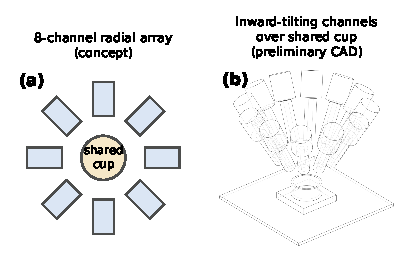
\includegraphics[width=8.3cm]{figures/fig6_future}
  \caption{Future work: the first multi-powder doser concept. (a) Eight channels arranged radially around a shared collection cup. (b) Preliminary CAD study of channels tilting inwards over the shared cup. The team set the concept and AI coding agents produced the CAD. The current multi-doser design moves passive auger cartridges on a roller chain past one fixed actuation and weighing station instead (repository issue \#128).}
  \label{fgr:future}
\end{figure}

\section*{Author contributions}
S.C.: conceptualization, methodology, investigation, CAD review, writing---original draft. W.M.: investigation, CAD review, validation. L.W.: investigation (electronics, PCB workflows), software. C.R.: investigation, hardware fabrication. G.E.: investigation, hardware fabrication. S.G.B.: conceptualization, supervision, funding acquisition, writing---review \& editing.

\section*{Conflicts of interest}
S.G.B. is a member of the \textit{Digital Discovery} advisory board. There are no other conflicts to declare.

\section*{Data availability}
All design files (parametric CAD source, STL files and renders), KiCad schematics, MicroPython firmware, AI prompt and response logs, the 97-entry design log, the raw test-protocol records and the analysis scripts are openly available at \url{https://github.com/vertical-cloud-lab/powder-doser}. The tidy datasets and scripts behind Figs.~\ref{fgr:conveyance}--\ref{fgr:closedloop} are in \texttt{paper/figures/}. Hardware designs are released under an open license (see the repository). The datasets will be deposited with a DOI on acceptance. References cited in the SI are listed in this article's reference list.

\section*{Acknowledgements}
This work was supported in part by a Utah NASA Space Grant Consortium undergraduate fellowship. Generative AI tools were used extensively and deliberately in this work, both as objects of study and as assistants. The GitHub Copilot coding agent and Claude-family models generated CAD code, firmware, analysis and figure scripts, and drafts and revisions of the manuscript text, all under human review; Edison Scientific was used for literature search and design review; and CADSmith and Zoo Design Studio (through its Zookeeper agent) were evaluated as text-to-CAD tools, with Zoo Design Studio adopted for the final parts. All AI use is logged in the public repository.

\balance

\renewcommand\refname{Notes and references}

\bibliography{references}
\bibliographystyle{rsc}

\end{document}
